\documentclass{beamer}
\usepackage{tikz,amsmath,hyperref,graphicx,stackrel,animate}
\usetikzlibrary{positioning,shadows,arrows,shapes,calc}
\newcommand{\argmax}{\operatornamewithlimits{argmax}}
\newcommand{\argmin}{\operatornamewithlimits{argmin}}
\mode<presentation>{\usetheme{Frankfurt}}
\AtBeginSection[]
{
  \begin{frame}<beamer>
    \frametitle{Outline}
    \tableofcontents[currentsection,currentsubsection]
  \end{frame}
}
\title{Lecture 5: Fourier Series and Discrete Fourier Transform}
\author{Mark Hasegawa-Johnson}
\date{ECE 401: Signal and Image Analysis, Fall 2020}  
\begin{document}

% Title
\begin{frame}
  \maketitle
\end{frame}

% Title
\begin{frame}
  \tableofcontents
\end{frame}

%%%%%%%%%%%%%%%%%%%%%%%%%%%%%%%%%%%%%%%%%%%%
\section[Review]{Review: Spectrum}
\setcounter{subsection}{1}

\begin{frame}
  \frametitle{Two-sided spectrum}

  The {\bf spectrum} of $x(t)$ is the set of frequencies, and their
  associated phasors,
  \[
  \mbox{Spectrum}\left( x(t) \right) =
  \left\{ (f_{-N},a_{-N}), \ldots, (f_0,a_0), \ldots, (f_N,a_N) \right\}
  \]
  such that
  \[
  x(t) = \sum_{k=-N}^N a_ke^{j2\pi f_kt}
  \]
\end{frame}

\begin{frame}
  \frametitle{Fourier's theorem}

  One reason the spectrum is useful is that {\bf\em any} periodic
  signal can be written as a sum of cosines.  Fourier's theorem says that
  any $x(t)$ that is periodic, i.e.,
  \[
  x(t+T_0) = x(t)
  \]
  can be written as
  \[
  x(t) = \sum_{k=-\infty}^\infty X_k e^{j2\pi k F_0 t}
  \]
  which is a special case of the spectrum for periodic signals:
  $f_k=kF_0$, and $a_k=X_k$, and
  \[
  F_0 = \frac{1}{T_0}
  \]
\end{frame}

\begin{frame}
  \frametitle{Analysis and Synthesis}

  \begin{itemize}
  \item {\bf Fourier Synthesis} is the process of generating the
    signal, $x(t)$, given its spectrum.  Last lecture, you learned
    how to do this, in general.
  \item {\bf Fourier Analysis} is the process of finding the spectrum,
    $X_k$, given the signal $x(t)$.  I'll tell you how to do that today.
  \end{itemize}
\end{frame}

%%%%%%%%%%%%%%%%%%%%%%%%%%%%%%%%%%%%%%%%%%%%
\section[Orthogonality]{Orthogonality}
\setcounter{subsection}{1}

\begin{frame}
  \frametitle{Orthogonality}

  Two functions $f(t)$ and $g(t)$ are said to be {\bf orthogonal}, over
  some period of time $T$, if
  \[
  \int_0^T f(t)g(t) = 0
  \]
\end{frame}

\begin{frame}
  \frametitle{Sine and Cosine are Orthogonal}

  For example, $\sin(2\pi t)$ and $\cos(2\pi t)$ are orthogonal over
  the period $0\le t\le 1$:
  \centerline{\includegraphics[height=2.5in]{exp/orthogonality_cos_sin.png}}
\end{frame}

\begin{frame}
  \frametitle{Sinusoids at Different Frequencies are Orthogonal}

  Similarly, sinusoids at different frequencies are orthogonal over any time
  segment that contains an integer number of periods:
  \centerline{\includegraphics[height=2.5in]{exp/orthogonality_3_4.png}}
\end{frame}

\begin{frame}
  \frametitle{How to use orthogonality}

  Suppose we have a signal that is known to be
  \[
  x(t) = a\cos(2\pi 3t)+b\sin(2\pi 3t)+c\cos(2\pi 4 t)+d\sin(2\pi 4t)+\ldots
  \]
  \ldots but we don't know $a$, $b$, $c$, $d$, etc.  Let's use
  orthogonality to figure out the value of $b$:
  \begin{align*}
    \int_0^1 x(t)\sin(2\pi 3t)dt &= 
    a\int_0^1 \cos(2\pi 3t)\sin(2\pi 3t)dt \\
    &+ b\int_0^1\sin(2\pi 3t)\sin(2\pi 3t)dt\\
    &+ c\int_0^1\cos(2\pi  4t)\sin(2\pi 3t)dt\\
    &+e\int_0^1\sin(2\pi 4t)\sin(2\pi 3t)dt+\ldots
  \end{align*}
\end{frame}

\begin{frame}
  \frametitle{How to use orthogonality}

  \ldots which simplifies to
  \[
  \int_0^1 x(t)\sin(2\pi 3t)dt
  = 0 + b\int_0^1\sin^2(2\pi 3t)dt + 0 + 0 + \ldots
  \]
  The average value of $\sin^2(t)$ is $1/2$, so
  \[
  \int_0^1 x(t)\sin(2\pi 3t)dt = \frac{b}{2}
  \]
  If we {\bf don't} know the value of $b$,
  but we {\bf do} know how to integrate $\int x(t)\sin(2\pi 3t)dt$,
  then we can find the value of $b$ from the formula above.
\end{frame}

\begin{frame}
  \frametitle{How to use orthogonality}
  \centerline{\includegraphics[height=2.5in]{exp/orthogonality_for_spectrum.png}}
\end{frame}

\begin{frame}
  \frametitle{How to use Orthogonality: Fourier Series}

  We still have one problem.  Integrating $\int x(t) \cos(2\pi 4t)dt$
  is hard---lots of ugly integration by parts and so on.  There are
  two useful solutions, depending on the situation:
  \begin{enumerate}
  \item {\bf Fourier Series:} Instead of cosine, use complex
    exponential:
    \[
    \int x(t) e^{-j2\pi ft} dt
    \]
    That integral is still hard, but it's always easier than $\int
    x(t) \cos(2\pi 4t)dt$.  It can usually be solved with some
    combination of integration by parts, variable substitution, etc.
  \item {\bf Discrete Fourier Transform:} Instead of integrating,
    write it as a sum:
    \[
    \sum x[n] e^{-j2\pi fn/F_s}
    \]
    \ldots and then write that as a line of python code, and solve it
    on the computer by typing {\tt np.sum()}.
  \end{enumerate}
\end{frame}
  
  
%%%%%%%%%%%%%%%%%%%%%%%%%%%%%%%%%%%%%%%%%%%%
\section[Fourier Series]{Fourier Series}
\setcounter{subsection}{1}

\begin{frame}
  \frametitle{Fourier's Theorem}

  Remember Fourier's theorem.  He said that any periodic signal, with
  a period of $T_0$ seconds, can be written
  \[
  x(t) = \sum_{k=-\infty}^\infty X_k e^{j2\pi kt/T_0}
  \]
\end{frame}

\begin{frame}
  \frametitle{Fourier's Theorem and Orthogonality}

  Take Fourier's theorem, and multiply both sides by $e^{-j2\pi \ell t/T_0}$:
  \[
  x(t)e^{-2\pi\ell t/T_0} = \sum_{k=-\infty}^\infty X_k e^{j2\pi (k-\ell)t/T_0}
  \]
  Now integrate both sides of that equation, over any complete period:
  \[
  \frac{1}{T_0}\int_0^{T_0}x(t)e^{-2\pi\ell t/T_0}dt =
  \sum_{k=-\infty}^\infty X_k \frac{1}{T_0}\int_0^{T_0} e^{j2\pi (k-\ell)t/T_0}dt
  \]
\end{frame}

\begin{frame}
  \frametitle{Fourier's Theorem and Orthogonality}

  Now think really hard about what's inside that integral sign:
  \begin{align*}
    &\frac{1}{T_0}\int_0^{T_0} e^{j2\pi (k-\ell)t/T_0}dt\\
    &=\frac{1}{T_0}\int_0^{T_0}\cos\left(\frac{2\pi(k-\ell)t}{T_0}\right)dt\\
    &+j\frac{1}{T_0}\int_0^{T_0}\sin\left(\frac{2\pi (k-\ell)t}{T_0}\right)dt
  \end{align*}
  \begin{itemize}
  \item If $k\ne\ell$, then we're integrating a cosine and a sine over
    $k-\ell$ periods.  That integral is always zero.
    \centerline{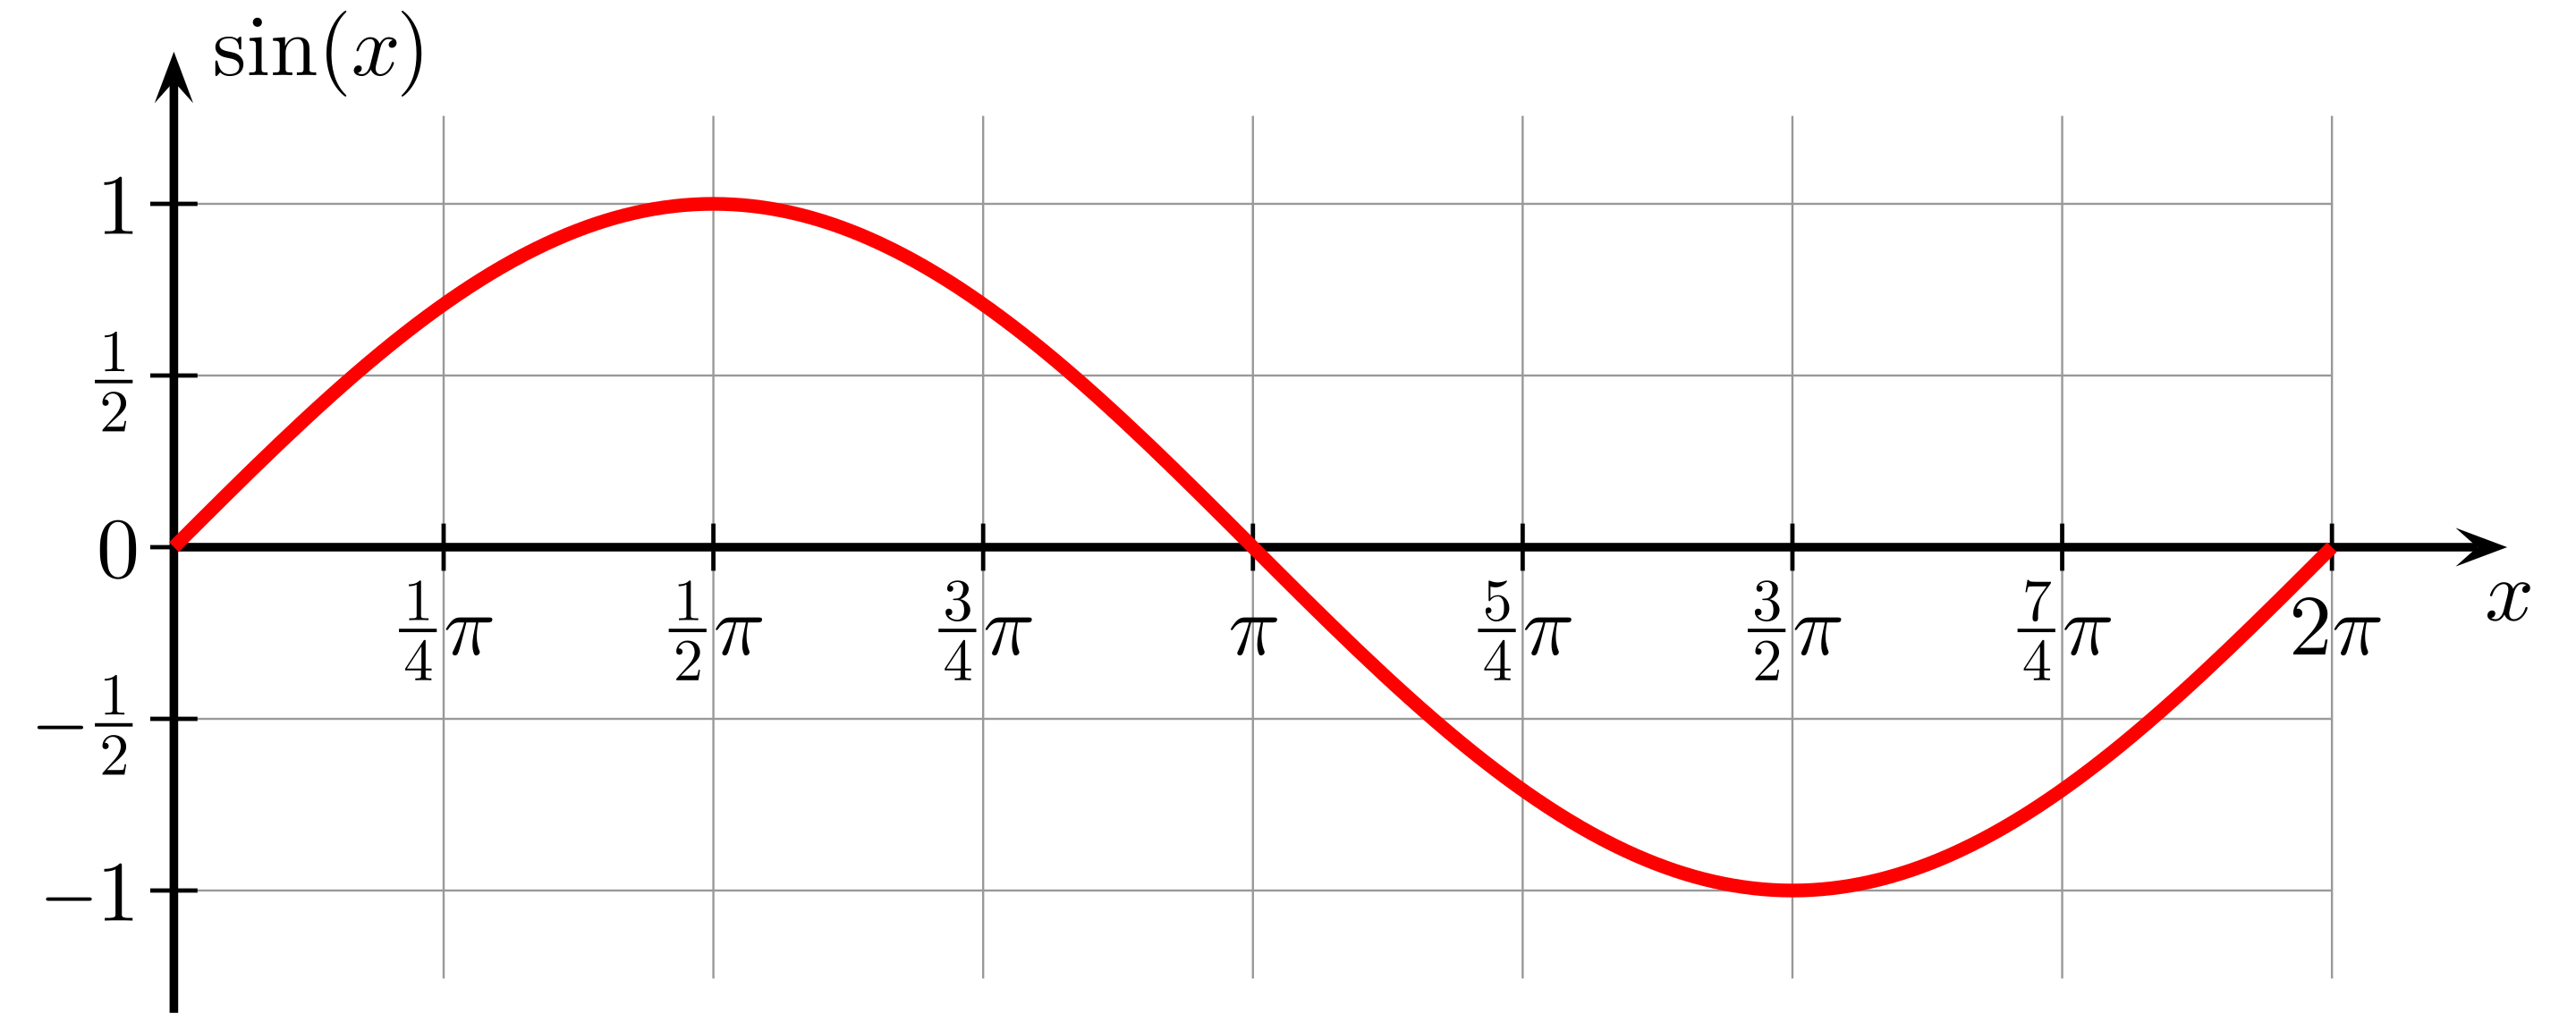
\includegraphics[height=0.25in]{Sine_one_period.png}}
  \item If $k=\ell$, then we're integrating
    \[
    \frac{1}{T_0}\int_0^{T_0}\cos(0)dt+
    +j\frac{1}{T_0}\int_0^{T_0}\sin(0)dt = 1
    \]
  \end{itemize}
\end{frame}

\begin{frame}
  \frametitle{Fourier Series: Analysis}

  So, because of orthogonality:
  \begin{align*}
  \frac{1}{T_0}\int_0^{T_0}x(t)e^{-2\pi\ell t/T_0}dt &=
  \sum_{k=-\infty}^\infty X_k \frac{1}{T_0}\int_0^{T_0} e^{j2\pi (k-\ell)t/T_0}dt\\
  &= \ldots + 0 + 0 + 0 + X_\ell + 0 +0 + 0 + \ldots
  \end{align*}
  
\end{frame}  

\begin{frame}
  \frametitle{Fourier Series}

  \begin{itemize}
  \item {\bf Analysis}  (finding the spectrum, given the waveform):
    \[
    X_k = \frac{1}{T_0}\int_0^{T_0} x(t)e^{-j2\pi kt/T_0}dt
    \]
  \item {\bf Synthesis} (finding the waveform, given the spectrum):
    \[
    x(t) = \sum_{k=-\infty}^\infty X_k e^{j2\pi kt/T_0}
    \]
  \end{itemize}
  
\end{frame}  

\begin{frame}
  \frametitle{Fourier series: Square wave example}
  \centerline{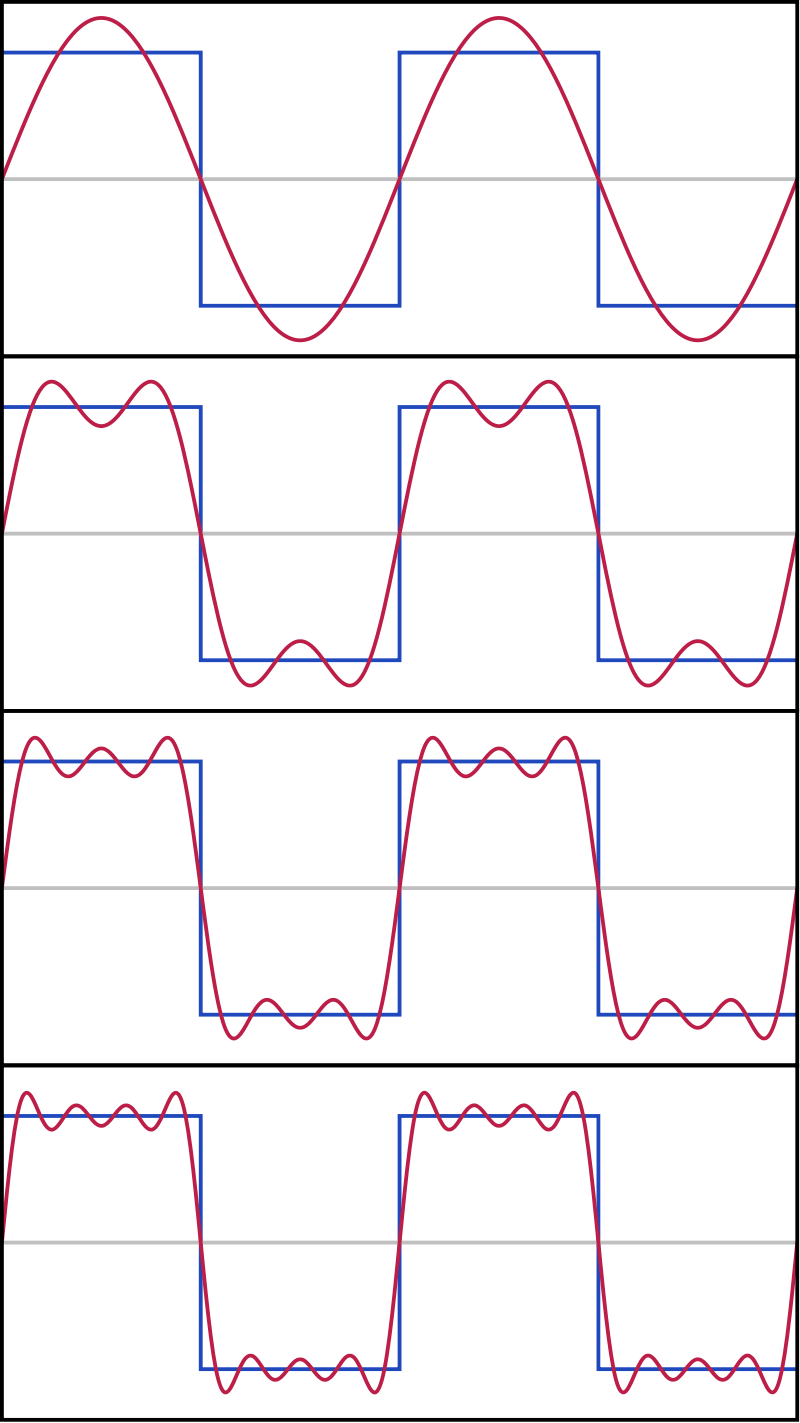
\includegraphics[height=2.5in]{../lec04/squarewave.png}}
\end{frame}

\begin{frame}
  \frametitle{Square wave: the $X_0$ term}
    \[
    X_0 = \frac{1}{T_0}\int_0^{T_0} x(t)e^{j2\pi 0 t/T_0}dt
    \]
  \centerline{\includegraphics[height=2.5in]{exp/fourierseries0.png}}
\end{frame}

\begin{frame}
  \frametitle{Square wave: the $X_1$ term}
    \[
    X_1 = \frac{1}{T_0}\int_0^{T_0} x(t)e^{j2\pi 1 t/T_0}dt
    \]
  \centerline{\includegraphics[height=2.5in]{exp/fourierseries1.png}}
\end{frame}

\begin{frame}
  \frametitle{Square wave: the $X_2$ term}
    \[
    X_2 = \frac{1}{T_0}\int_0^{T_0} x(t)e^{j2\pi 2 t/T_0}dt
    \]
  \centerline{\includegraphics[height=2.5in]{exp/fourierseries2.png}}
\end{frame}

\begin{frame}
  \frametitle{Square wave: the $X_3$ term}
    \[
    X_3 = \frac{1}{T_0}\int_0^{T_0} x(t)e^{j2\pi 3 t/T_0}dt
    \]
  \centerline{\includegraphics[height=2.5in]{exp/fourierseries3.png}}
\end{frame}

\begin{frame}
  \frametitle{Square wave: the $X_5$ term}
    \[
    X_5 = \frac{1}{T_0}\int_0^{T_0} x(t)e^{j2\pi 5 t/T_0}dt
    \]
  \centerline{\includegraphics[height=2.5in]{exp/fourierseries5.png}}
\end{frame}

\begin{frame}
  \frametitle{Fourier Series}

  \begin{itemize}
  \item {\bf Analysis}  (finding the spectrum, given the waveform):
    \[
    X_k = \frac{1}{T_0}\int_0^{T_0} x(t)e^{-j2\pi kt/T_0}dt
    \]
  \item {\bf Synthesis} (finding the waveform, given the spectrum):
    \[
    x(t) = \sum_{k=-\infty}^\infty X_k e^{j2\pi kt/T_0}
    \]
  \end{itemize}
  
\end{frame}  


%%%%%%%%%%%%%%%%%%%%%%%%%%%%%%%%%%%%%%%%%%%%
\section[DFT]{Discrete Fourier Tranform}
\setcounter{subsection}{1}

\begin{frame}
  \frametitle{Discrete-time Fourier Series}

  Suppose you have a signal $x[n]$, sampled at a certain number of samples per second.
  Suppose $x[n]$ is periodic with a period of $N$ samples, i.e.,
  \[
  x[n] = x[n+N]
  \]
  Then
  \[
  x[n] = \sum_{k=0}^{N-1} X_k e^{j2\pi kn/N}
  \]
\end{frame}

\begin{frame}
  \frametitle{Discrete Fourier Transform}

  Suppose you have a signal $x[n]$, sampled at a certain number of
  samples per second.  We'll pretend that $x[n]$ is periodic with a
  period of $N$ samples (even if it's not really), i.e., we'll pretend
  that
  \[
  x[n] = x[n+N]
  \]
  We'll define $X[k]$ so that
  \[
  x[n] = \frac{1}{N}\sum_{k=0}^{N-1} X[k] e^{j2\pi kn/N}
  \]
  \ldots in other words, the DFT is just a scaled-up  Fourier series.
\end{frame}

\begin{frame}
  \frametitle{Fourier's Theorem and Orthogonality}

  Take Fourier's theorem, and multiply both sides by $e^{-j2\pi \ell n/N}$:
  \[
  x[n]e^{-2\pi\ell n/N} = \frac{1}{N}\sum_{k=0}^{N-1} X[k] e^{j2\pi (k-\ell)n/N}
  \]
  Now sum both sides of that equation:
  \[
  \sum_{n=0}^{N-1}x[n]e^{-2\pi\ell n/N} =
  \frac{1}{N}\sum_{k=0}^{N-1} X[k] \sum_{n=0}^{N-1} e^{j2\pi (k-\ell)n/N}
  \]
\end{frame}

\begin{frame}
  \frametitle{Fourier's Theorem and Orthogonality}

  Now think really hard about what's inside that summation:
  \begin{align*}
    &\sum_{n=0}^{N-1} e^{j2\pi (k-\ell)n/N}dt\\
    &=\sum_{n=0}^{N-1}\cos\left(\frac{2\pi(k-\ell)n}{N}\right)
    +j\sum_{n=0}^{N-1}\sin\left(\frac{2\pi (k-\ell)n}{N}\right)
  \end{align*}
  \begin{itemize}
  \item If $k\ne\ell$, then we're summing a cosine and a sine over
    $k-\ell$ periods.  That sum is always zero.
    \centerline{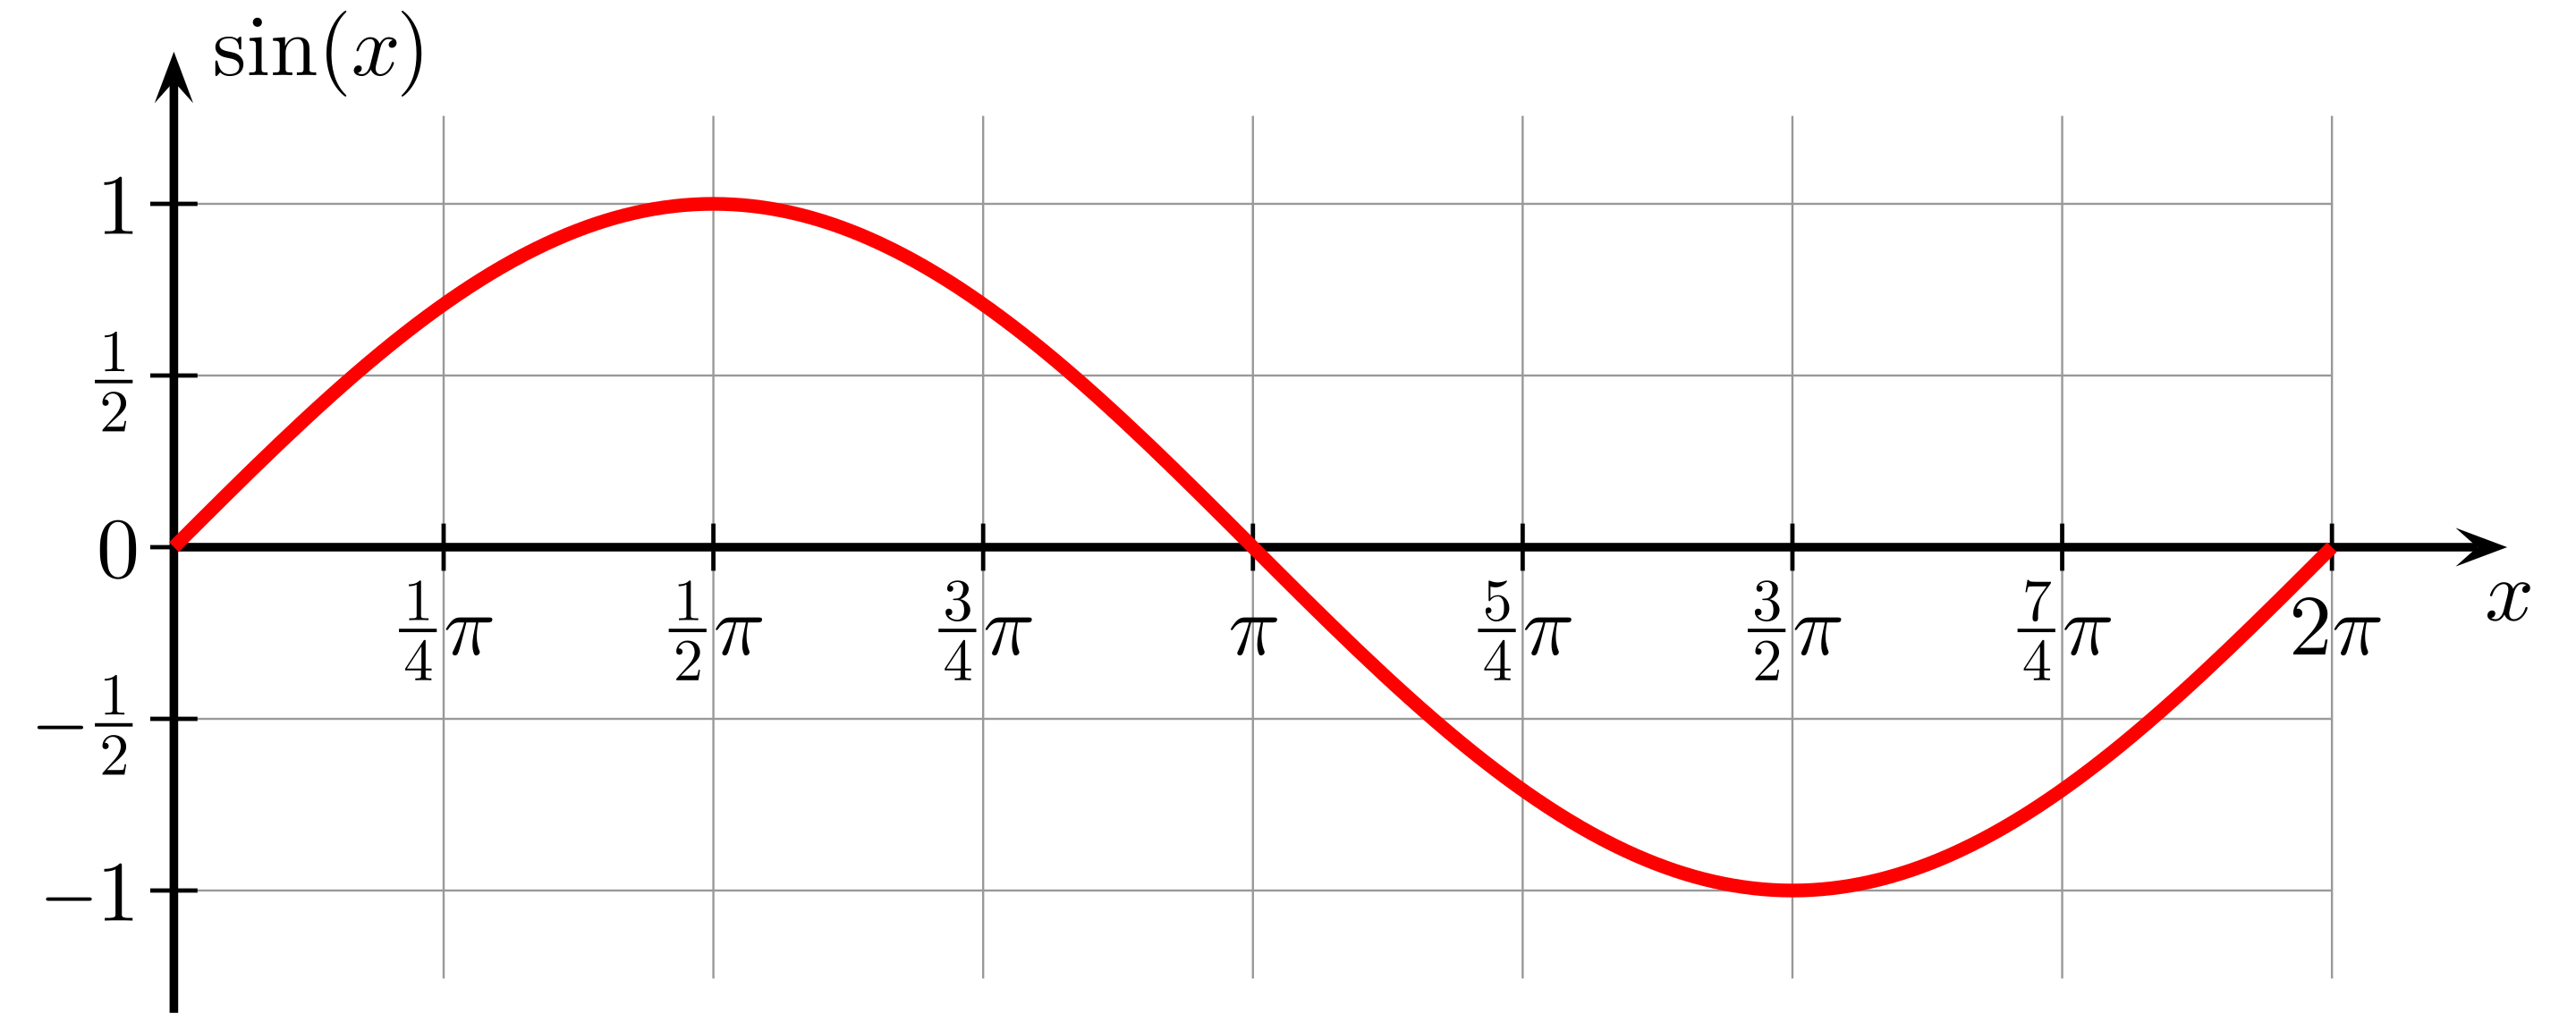
\includegraphics[height=0.25in]{Sine_one_period.png}}
  \item If $k=\ell$, then we're summing
    \[
    \sum_{n=0}^{N-1}\cos(0)+
    +j\sum_{n=0}^{N-1}\sin(0) = N
    \]
  \end{itemize}
\end{frame}

\begin{frame}
  \frametitle{DFT: Analysis}

  So, because of orthogonality:
  \begin{align*}
  \sum_{n=0}^{N-1}x[n]e^{-2\pi\ell n/N} &=
  \frac{1}{N}\sum_{k=0}^{N-1} X[k]\sum_{n=0}^{N-1} e^{j2\pi (k-\ell)n/N}\\
  &= 0+ 0+ \ldots + 0 + 0 + X[\ell] + 0 +0 + \ldots + 0 + 0
  \end{align*}
  
\end{frame}  

\begin{frame}
  \frametitle{Discrete Fourier Transform}

  \begin{itemize}
  \item {\bf Analysis}  (finding the spectrum, given the waveform):
    \[
    X[k] = \sum_{n=0}^{N-1} x[n]e^{-j2\pi kn/N}
    \]
  \item {\bf Synthesis} (finding the waveform, given the spectrum):
    \[
    x[n] = \frac{1}{N}\sum_{k=0}^{N-1} X[k] e^{j2\pi kn/N}
    \]
  \end{itemize}
  
\end{frame}  


%%%%%%%%%%%%%%%%%%%%%%%%%%%%%%%%%%%%%%%%%%%%
\section[Summary]{Summary}
\setcounter{subsection}{1}

\begin{frame}
  \frametitle{Summary}
  \begin{itemize}
  \item {\bf Analysis}  (finding the spectrum, given the waveform):
    \[
    X_k = \frac{1}{T_0}\int_0^{T_0} x(t)e^{-j2\pi kt/T_0}dt
    \]
  \item {\bf Synthesis}  (finding the waveform, given the spectrum):
    \[
    x(t) = \sum_{k=-\infty}^\infty X_k e^{j2\pi kt/T_0}
    \]
  \item {\bf DFT Analysis}  (finding the spectrum, given the waveform):
    \[
    X[k] = \sum_{n=0}^{N-1} x[n]e^{-j2\pi kn/N}
    \]
  \item {\bf DFT Synthesis} (finding the waveform, given the spectrum):
    \[
    x[n] = \frac{1}{N}\sum_{k=0}^{N-1} X[k] e^{j2\pi kn/N}
    \]
  \end{itemize}
\end{frame}  
    
\begin{frame}
  \frametitle{Summary}
  Things you should know, from today's lecture:
  \begin{itemize}
  \item You don't need to memorize the equations on the previous page,
    but, for example, given the synthesis equation, you should be able
    to apply the orthogonality principle to derive the corresponding
    analysis equation.
  \item You should know that every periodic signal $x[n]$ has a
    spectrum $X[k]$, and that you can use {\tt np.fft.fft} to compute
    it.
  \item You should know that the DFT makes an implicit assumption that
    the signal is periodic with a period of $N$ samples.  If the
    signal isn't really periodic, then you might get weird artifacts
    because of that assumption -- minor at most time scales, but
    important for careful music analysis.
  \end{itemize}
\end{frame}
        
\end{document}
